\section*{Problem 1}


\[
p=\rho RT,\qquad h=c_pT,\qquad
\gamma=1.4,\quad R=287~\mathrm{J/(kg\,K)},\quad
c_p=\frac{\gamma R}{\gamma-1}=1004.5~\mathrm{J/(kg\,K)}.
\]
% L3 notes PDF p.1, Eqs. (72)--(74); p.2, cp-cv=R above Eq. (77).
$M_1=0.25$, $T_1=300~\mathrm{K}$, $p_1=100~\mathrm{kPa}$, and $A_1=0.10~\mathrm{m^2}$.


\partlabel{(a)}
% L7 notes PDF p.2, Eqs. (139), (141)--(142): stagnation enthalpy.
% L3 notes PDF p.2, Eq. (77), integrated with constant cp and s0=s.
\[
h_0=c_pT+\frac{u^2}{2}=c_pT_0,\qquad
s_0=s\quad\Longrightarrow\quad
c_p\ln\frac{T_0}{T}-R\ln\frac{p_0}{p}=0.
\]
% L9 notes PDF p.2, unnumbered relations immediately before Eq. (11).
% L10 notes PDF p.8, Eq. (101); L12 notes PDF p.2, Eq. (237).
\begin{align*}
a_1&=\sqrt{\gamma RT_1}=\sqrt{1.4(287)(300)}
=\boxed{347.189~\mathrm{m/s}},\\
u_1&=M_1a_1=0.25(347.1887)=\boxed{86.7972~\mathrm{m/s}},\\
T_{0,1}&=T_1\left(1+\frac{\gamma-1}{2}M_1^2\right)
=300[1+0.2(0.25)^2]=\boxed{303.750~\mathrm{K}},\\
p_{0,1}&=p_1\left(\frac{T_{0,1}}{T_1}\right)^{\gamma/(\gamma-1)}
=100\left(\frac{303.75}{300}\right)^{3.5}
=\boxed{104.444~\mathrm{kPa}}.
\end{align*}
% L12 notes PDF p.1, Eq. (228), defines the isentropic area-Mach relation.
\[
\frac{A}{A^*}=F(M)\equiv\frac{1}{M}
\left[\frac{2}{\gamma+1}\left(1+\frac{\gamma-1}{2}M^2\right)\right]
^{\frac{\gamma+1}{2(\gamma-1)}}.
\]
% L12 notes PDF p.1, Eq. (223): mass conservation.
\begin{align*}
\frac{A_1}{A_1^*}&=F(0.25)=\boxed{2.402710},\qquad
A_1^*=\frac{0.10}{2.40270996}=\boxed{0.0416197~\mathrm{m^2}},\\
\dot m&=\rho_1u_1A_1=\frac{p_1}{RT_1}u_1A_1
=\frac{100000}{287(300)}(86.797177)(0.10)
=\boxed{10.0810~\mathrm{kg/s}}.
\end{align*}

\partlabel{(b)}

% L10 notes PDF p.2, Eqs. (47)--(49); p.9, Eq. (108).
\[
\rho u=\mathrm{const.},\qquad p+\rho u^2=\mathrm{const.},\qquad
q=h_0^*-h_{0,1}=c_p(T_0^*-T_{0,1}).
\]
$\rho u^2=\gamma pM^2，M^*=1$,
% L10 notes PDF p.7, Eqs. (91), (93), and (96); rearranged at state 1.
\begin{align*}
p_1(1+\gamma M_1^2)&=p^*(1+\gamma),\\
p^*&=p_1\frac{1+\gamma M_1^2}{1+\gamma}
=100\frac{1+1.4(0.25)^2}{2.4}=\boxed{45.3125~\mathrm{kPa}},\\
\frac{p_1M_1}{\sqrt{T_1}}&=\frac{p^*}{\sqrt{T^*}}
\quad\Longrightarrow\quad
T^*=T_1\left(\frac{p^*}{p_1M_1}\right)^2
=300\left(\frac{45.3125}{100(0.25)}\right)^2
=\boxed{985.547~\mathrm{K}},\\
a^*&=\sqrt{\gamma RT^*}=\sqrt{1.4(287)(985.546875)}
=\boxed{629.280~\mathrm{m/s}}.
\end{align*}
% L10 notes PDF p.8, Eq. (101); L12 notes PDF p.2, Eq. (237), at M=1.
\begin{align*}
T_0^*&=T^*\frac{\gamma+1}{2}=1.2(985.546875)
=\boxed{1182.656~\mathrm{K}},\\
p_0^*&=p^*\left(\frac{\gamma+1}{2}\right)^{\gamma/(\gamma-1)}
=45.3125(1.2)^{3.5}=\boxed{85.7734~\mathrm{kPa}},\\
q&=1004.5(1182.65625-303.75)~\mathrm{J/kg}
=882861.328~\mathrm{J/kg}\\
&=\frac{882861.328}{1000}~\mathrm{kJ/kg}
=\boxed{882.861~\mathrm{kJ/kg}}.
\end{align*}
\[
\boxed{M^*=1,\qquad A^*=A_1=0.100000~\mathrm{m^2},\qquad
\dot m=10.0810~\mathrm{kg/s}.}
\]


\partlabel{(c)}

% L11 notes PDF p.1, Eqs. (118)--(119); p.5, Eqs. (160)--(162).
\[
\rho u=\mathrm{const.},\qquad h_0=c_pT+\frac{u^2}{2}=\mathrm{const.}
\quad\Longrightarrow\quad T_0^*=T_{0,1}.
\]
\begin{align*}
T^*&=\frac{T_{0,1}}{(\gamma+1)/2}
=\frac{303.75}{1.2}=\boxed{253.125~\mathrm{K}},\\
p^*&=p_1M_1\sqrt{\frac{T^*}{T_1}}
=100(0.25)\sqrt{\frac{253.125}{300}}
=\boxed{22.9640~\mathrm{kPa}},\\
a^*&=\sqrt{\gamma RT^*}=\boxed{318.913~\mathrm{m/s}},\qquad
p_0^*=p^*(1.2)^{3.5}=\boxed{43.4692~\mathrm{kPa}}.
\end{align*}
\[
\boxed{T_0^*=303.750~\mathrm{K},\qquad A^*=0.100000~\mathrm{m^2},\qquad
\dot m=10.0810~\mathrm{kg/s}.}
\]


\partlabel{(d)}

% L12 notes PDF p.1, Eq. (228); p.2, Eqs. (233), (237).
\begin{align*}
T^*&=\frac{T_{0,1}}{1.2}=\boxed{253.125~\mathrm{K}},\qquad
a^*=\sqrt{\gamma RT^*}=\boxed{318.913~\mathrm{m/s}},\\
p^*&=\frac{p_{0,1}}{(1.2)^{3.5}}
=\frac{104.443787}{(1.2)^{3.5}}=\boxed{55.1758~\mathrm{kPa}},\\
T_0^*&=\boxed{303.750~\mathrm{K}},\qquad
p_0^*=\boxed{104.444~\mathrm{kPa}},\\
A^*&=A_1^*=\boxed{0.0416197~\mathrm{m^2}},\qquad
\dot m=\boxed{10.0810~\mathrm{kg/s}}.
\end{align*}

\partlabel{(e)}
% L9 notes PDF p.4, Eq. (25): entropy difference; its shock-specific >0
% is not imposed on the isentropic process. L3 notes PDF p.1 Eq. (74): h datum.
\[
h=c_pT,\qquad \Delta s=s-s_1
=c_p\ln\frac{T}{T_1}-R\ln\frac{p}{p_1}.
\]
The plotted states are parameterized by $0.25\le M\le1$:
% Rayleigh: L10 notes PDF p.7, Eqs. (91), (96), expressed relative to state 1.
% Fanno: L11 notes PDF p.5, Eqs. (160), (161), expressed relative to state 1.
% Isentropic: L10 notes PDF p.8 Eq. (101); L12 notes PDF p.2 Eq. (237).
\begin{align*}
\text{Rayleigh:}\qquad
p_R(M)&=p_1\frac{1+\gamma M_1^2}{1+\gamma M^2},&
T_R(M)&=T_1\left(\frac{p_R(M)M}{p_1M_1}\right)^2,\\
\text{Fanno:}\qquad
T_F(M)&=\frac{T_{0,1}}{1+0.2M^2},&
p_F(M)&=p_1\frac{M_1}{M}\sqrt{\frac{T_F(M)}{T_1}},\\
\text{Isentropic:}\qquad
T_I(M)&=\frac{T_{0,1}}{1+0.2M^2},&
p_I(M)&=\frac{p_{0,1}}{(1+0.2M^2)^{3.5}}.
\end{align*}
\begin{center}
\begin{tabular}{lrrrr}
\hline
State & $\Delta s$ [J/(kg K)] & $h$ [kJ/kg] & $T$ [K] & $p$ [kPa] \\
\hline
Initial & 0 & 301.350 & 300.000 & 100.000 \\
Rayleigh sonic & 1421.952 & 989.982 & 985.547 & 45.3125 \\
Fanno sonic & 251.583 & 254.264 & 253.125 & 22.9640 \\
Isentropic sonic & 0 & 254.264 & 253.125 & 55.1758 \\
\hline
\end{tabular}
\end{center}
\begin{center}
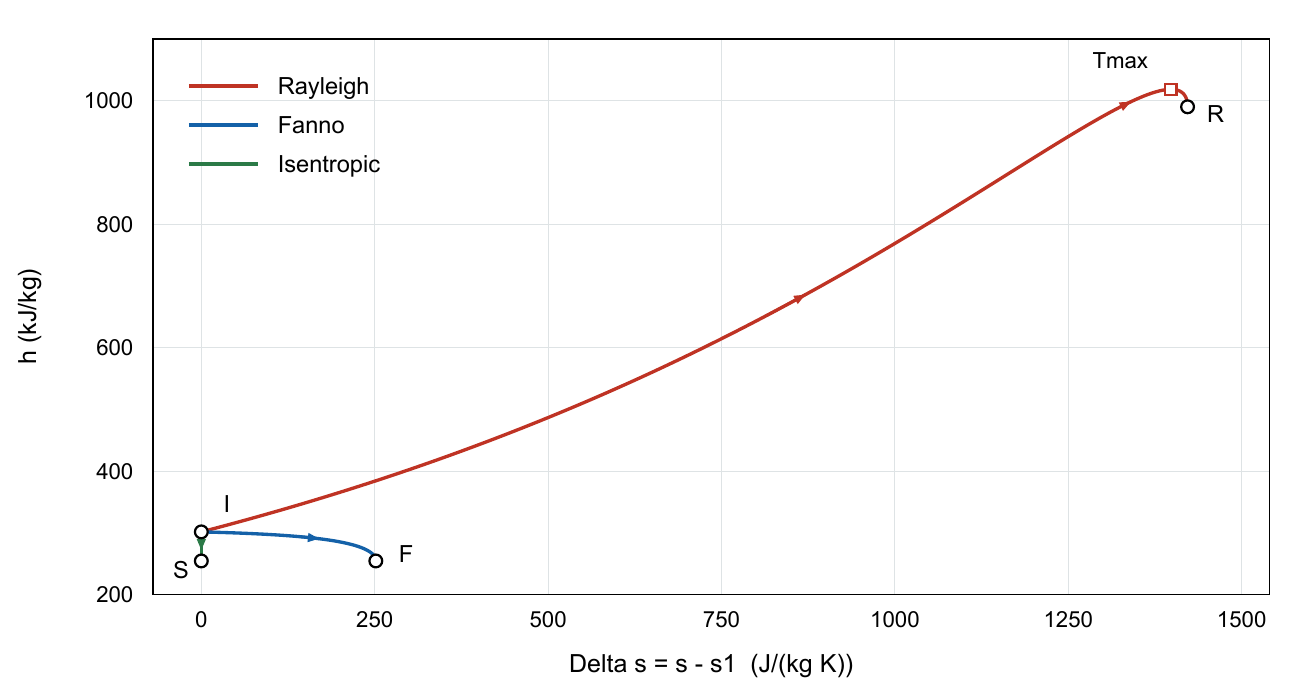
\includegraphics[width=0.80\linewidth]{figures/HW3_Problem1_hs.png}
\end{center}
% L10 notes PDF p.5, Eqs. (74)--(75): maximum static h at M=1/sqrt(gamma).
For Rayleigh flow, $h$ is maximum at $M=1/\sqrt{\gamma}=0.845154$:
$T=1013.705~\mathrm{K}$ and $h=1018.267~\mathrm{kJ/kg}$.
Further heating increases $T_0$ while $T$ decreases to the sonic value.

\partlabel{(f)}
Rayleigh heating increases $T_0$ and decreases $p_0$; neither stagnation quantity is constant.
Fanno friction preserves $T_0$ and decreases $p_0$.
Isentropic contraction preserves both $T_0$ and $p_0$.
The condition $M=1$ specifies $u=a$, not a unique thermodynamic state.
Fanno and isentropic flow have the same sonic $T$ because they preserve the same $T_0$,
but friction produces a different entropy, sonic pressure, and required sonic area.
